\documentclass[11pt,handout]{beamer}
\usepackage[latin1]{inputenc}
\usepackage{amsmath}
\usepackage{framed}
\usepackage{listings}
% Graphics packages
\usepackage{graphicx}
\graphicspath{{figures/}}
\usepackage{pgf}
% Table packages
\usepackage{booktabs}
\usepackage{multirow}
\usepackage{tabularx}

\usetheme{Singapore}
\title[Changepoints in Open Source Evolution]{An Exploratory Study of Project Activity Changepoints in Open Source Software Evolution}
% \author[Walden]{James~Walden\\Center for Information Security\\Northern Kentucky University\\waldenj@nku.edu}
\author[]{James Walden \textsuperscript{1} \and Noah Burgin \inst{2} \and Kuljit Kaur\inst{3}}
\institute[]{\textsuperscript{1} Northern Kentucky University \and \inst{2} %
   University of Tennessee, Knoxville \and \inst{3} Guru Nanak Dev University} 
\date{}

% Setup logo with if statement to control placement
\newif\ifplacelogo % create a new conditional
\placelogotrue % set it to true
% Customize footline with NKU logo and no navigation symbols
% \logo{\ifplacelogo
%   \includegraphics[width=2cm, height=2cm, keepaspectratio]{nku-logo.jpg}~%
% \fi}

% Remove navigation circles for each slide below section names
\setbeamertemplate{navigation symbols}{}
\setbeamertemplate{mini frames}{}

% Add numbers in table of contents
\setbeamertemplate{section in toc}[sections numbered]

\begin{document}
\begin{frame}
    \titlepage
\end{frame}

\begin{frame}{Software Evolution: Continuous or Punctuated?}
    Changepoints are when statistical properties of time series change.\\
    \vskip 3 mm
    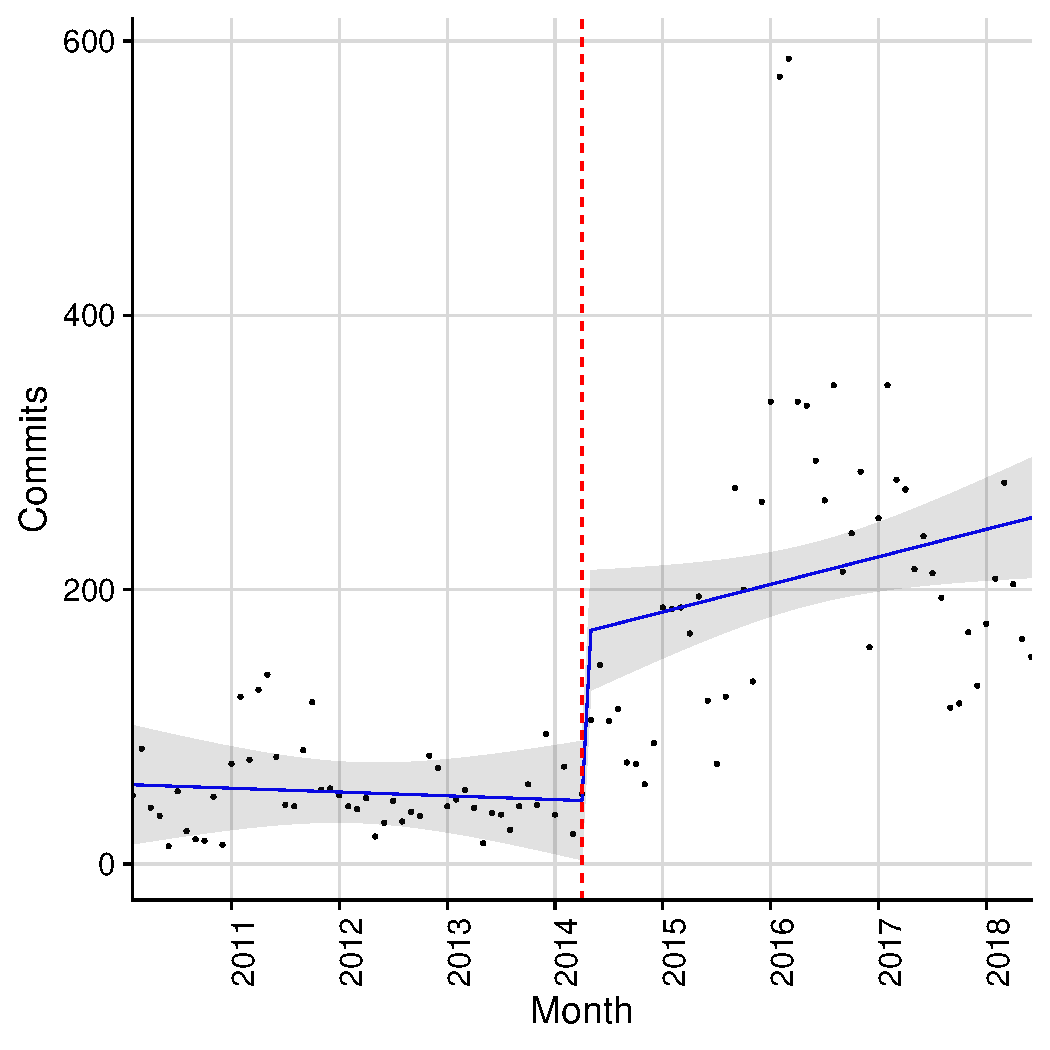
\includegraphics[width=0.5\textwidth,keepaspectratio]{ncommits.pdf}%
    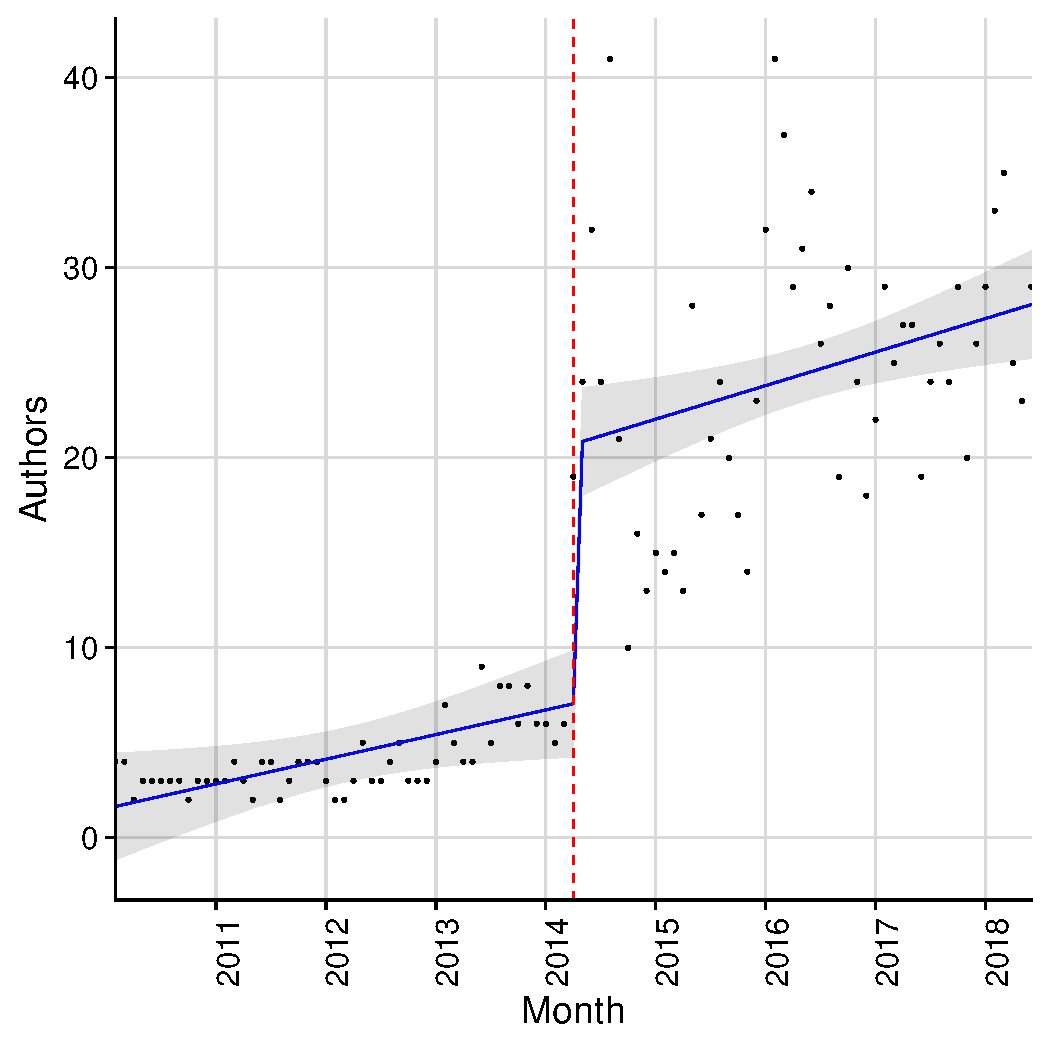
\includegraphics[width=0.5\textwidth,keepaspectratio]{nauthors.pdf}
\end{frame}

\begin{frame}{Research Questions}
    Exploratory Research Questions:
    \begin{enumerate}
        \item How common are changepoints in open source project activity?
        \item What are the signs and magnitudes of changes at changepoints?
    \end{enumerate}
    \vskip 3 mm
    Future Research Questions:
    \begin{enumerate}
        \item Can we identify changepoints that indicate project events?
        \item Can we find changepoint patterns indicative of lifecycles?
    \end{enumerate}
\end{frame}

\begin{frame}{Data Collection}
World of Code is an archive of 120+ million git repositories.\\
\vskip 5 mm
Selected projects that met the following criteria from WoC:
    \begin{itemize}
        \item At least 48 months between the first and last commit.
        \item At least 5000 commits.
        \item At least 50 authors.
    \end{itemize}
\vskip 3 mm
We found 8,919 projects that met these criteria.
\end{frame}

% Talking points:
%    * 99.6% have changepoints (32 projects do not)
%    * Median number of changepoints is 3
%    * 90% have between one and six changepoints.
%    * 27 projects have 10 or more changepoints
%
\begin{frame}{Projects by Number of Changepoints in Commits}
    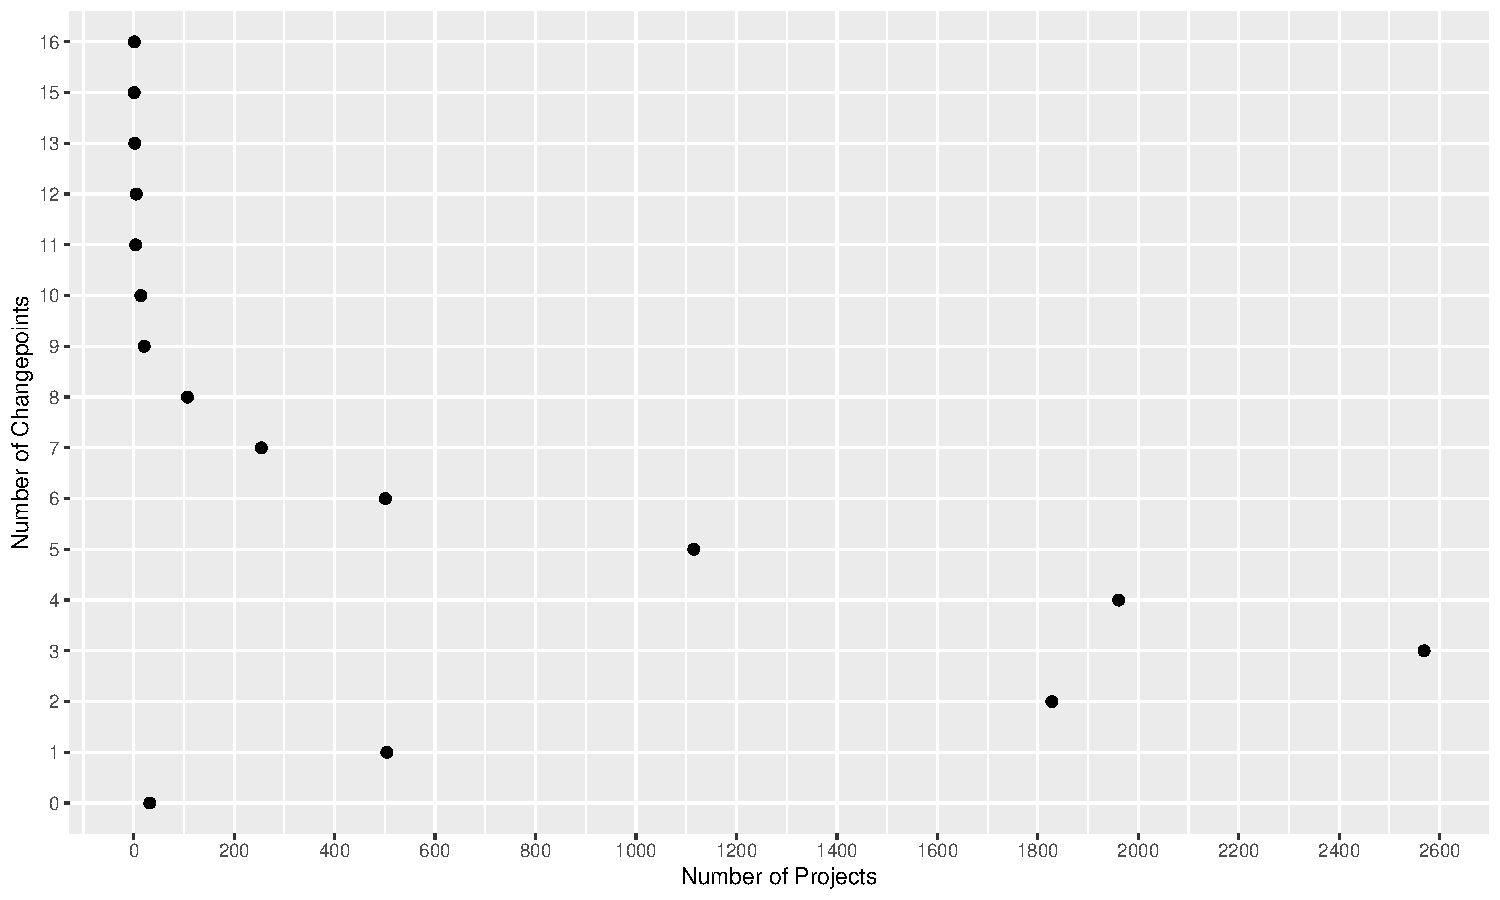
\includegraphics[width=\textwidth,keepaspectratio]{commit-changepoints.pdf}
\end{frame}

% We found a total of 31,416 changepoints in project commit
%    * 49% (15,342) were increases in commit activity 
%    * 51% (16,047) were reductions in activity. 
% We computed the magnitude of a changepoint as the difference in 
% means in the number of monthly commits before and after the
% changepoint. 
%
% The size of most changes were relatively small
%    * IQR ranges between -75 to 87 commits per month
% Some outliers are very large as can be seen long tails in figure.
%
\begin{frame}{Size of Changes in Commit Time Series}
    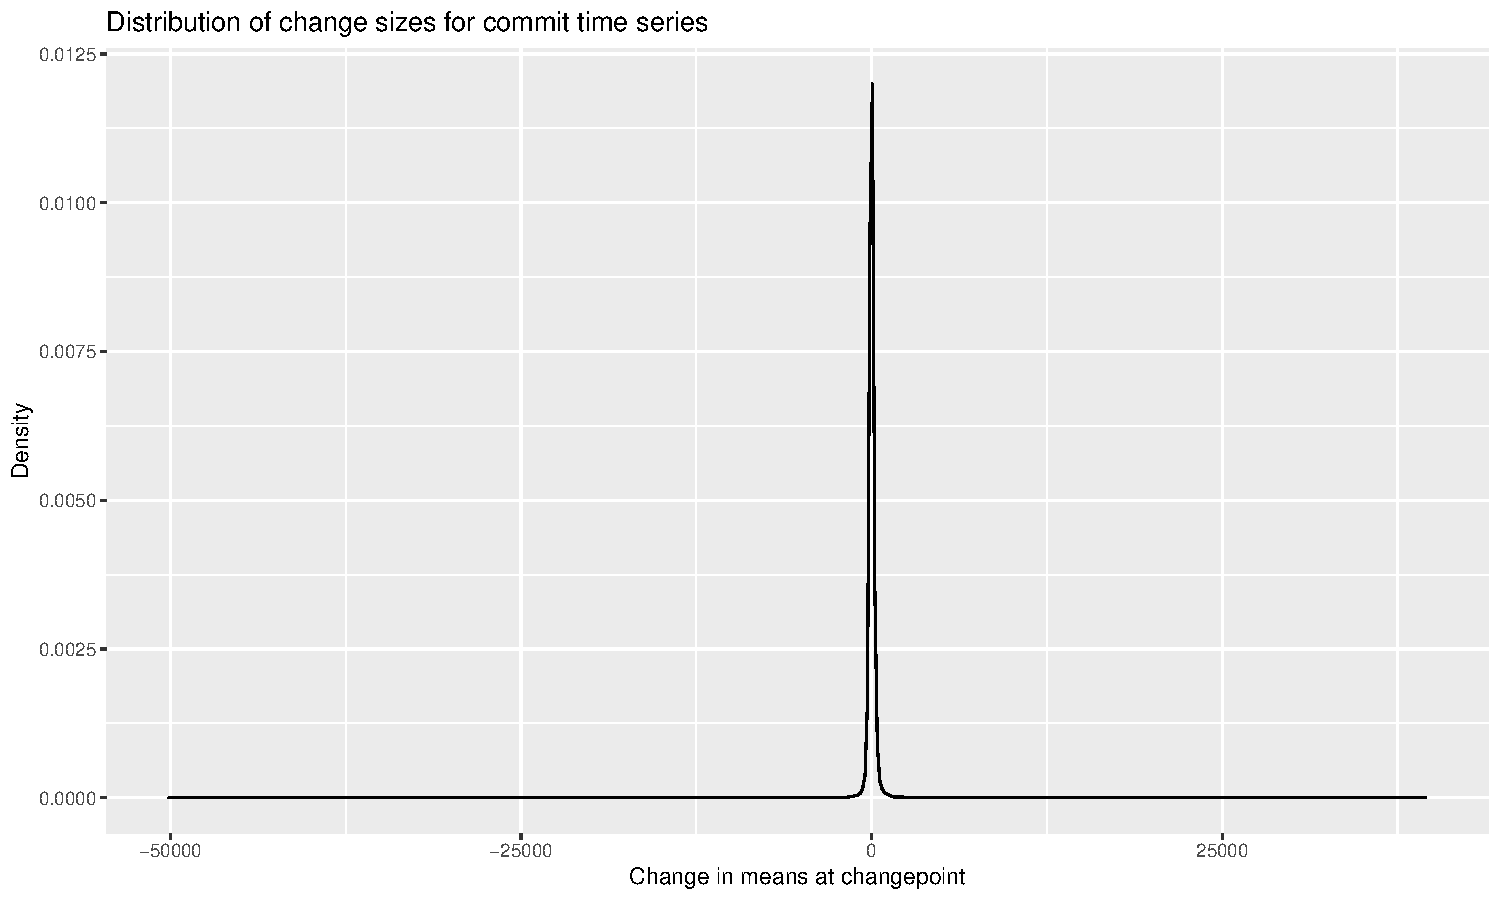
\includegraphics[width=\textwidth,keepaspectratio]{commit-changesizes.pdf}
\end{frame}

\begin{frame}{Conclusions and Future Work}
    Conclusions:
    \begin{itemize}
        \item Over 99\% of open source projects with extensive history have changepoints.
        \item Increases and decreases in project activity occur in roughly equal shares (51\% vs 49\%).
        \item Majority of changepoints range from -75 to 87 commits/month, but there are a number of huge outliers.
    \end{itemize}
    \vskip 5mm
    \textbf{Paper:} \url{https://arxiv.org/abs/2103.11013}
    \vskip 5mm
    \textbf{Code and Data:} \url{https://github.com/woc-hack/inflection-points}
    \vskip 5mm
    % Future Work:
    % \begin{itemize}
    %     \item Identify changepoint patterns, with a goal of finding lifecycle models.
    %     \item Determine the impact of external events like COVID-19 on open source evolution.
    %     \item Examine changepoints in static code metrics.
    % \end{itemize}
\end{frame}

\end{document}
